\chapter{Background and Theory}
\label{chp:background}

Vector graphics have been popular in the computer industry for many years,
seeing frequent use in analogue oscilloscopes, video arcade games \cite{astroids},
and as display devices for computers \cite{ibm2250}\cite{tektronix4010}.
This chapter introduces the concept of vector graphics, and compares it to its counterpart, raster graphics.

\section{Computer Graphics}
Computer graphics, introduced around 1960 \cite[sec. 1.1.1]{graphics-visualization-algorithms}, is the huge branch in today's computing world that deals with imagery and animations produced by a computer.
At its core, this project deals with the type of computer graphics defined as vector graphics, which is detailed further in this section.
As the project involves what is known as raster graphics, the report includes raster graphics theory as well.

\subsection{2D Raster Graphics}
Raster graphics are also known as bitmap graphics, and consist of a two-dimensional array of discrete values, where each discrete value is used to describe the color of the pixel at a given position in the array.
A bitmap image is often represented in the RGB color scheme - that is where you define different levels of red, green and blue for each pixel until you are able to render the correct color.

To display a full image, the computer needs to store \( (width \times height) \times RGB \) bits.
Today, RGB usually contains 3 bytes, one byte for each color, and a resolution of \(1920 \times 1080\) pixels (Full HD) is becoming the standard.
With this resolution, a single image therefore requires about 6 MB to store.
There exists method to compress images, such as different file formats. 
However, raster images still uses a significant amount of space.

A good thing with raster graphics is that it can be used to store any image, and still keep almost any level of detail intact. 
Should you need to increase the detail in an image, you just increase the pixel count accordingly. 
A common use case is storing photographs and images used on the web. 
In today's computing world, raster graphics is the dominating paradigm, and almost all digital 2D graphics you encounter are stored in a rasterized format, such as \texttt{.jpeg}, \texttt{.png} and \texttt{.gif}.
\subsection{2D Vector Graphics}
Vector graphics is a form of computer graphics where mathematical expressions are used to describe an image.
The image, or the 'scene', is made up of primitives that describe paths, lines and curves, and sometimes combinations of these in order to create more complex shapes.

By relying on mathematical expressions instead of pixel values relative to screen resolution, vector graphics can be described as resolution independent.
This is often conceptualized in the form of scaling:
While scaling a rasterized image will result in a blurry image, scaling a vectorized image will result in the mathematical expressions being recalculated, and the image will remain sharp.
The scaling process is visualized in Figure \ref{fig:vectorscaling}.

\begin{figure}[h!]
\centering 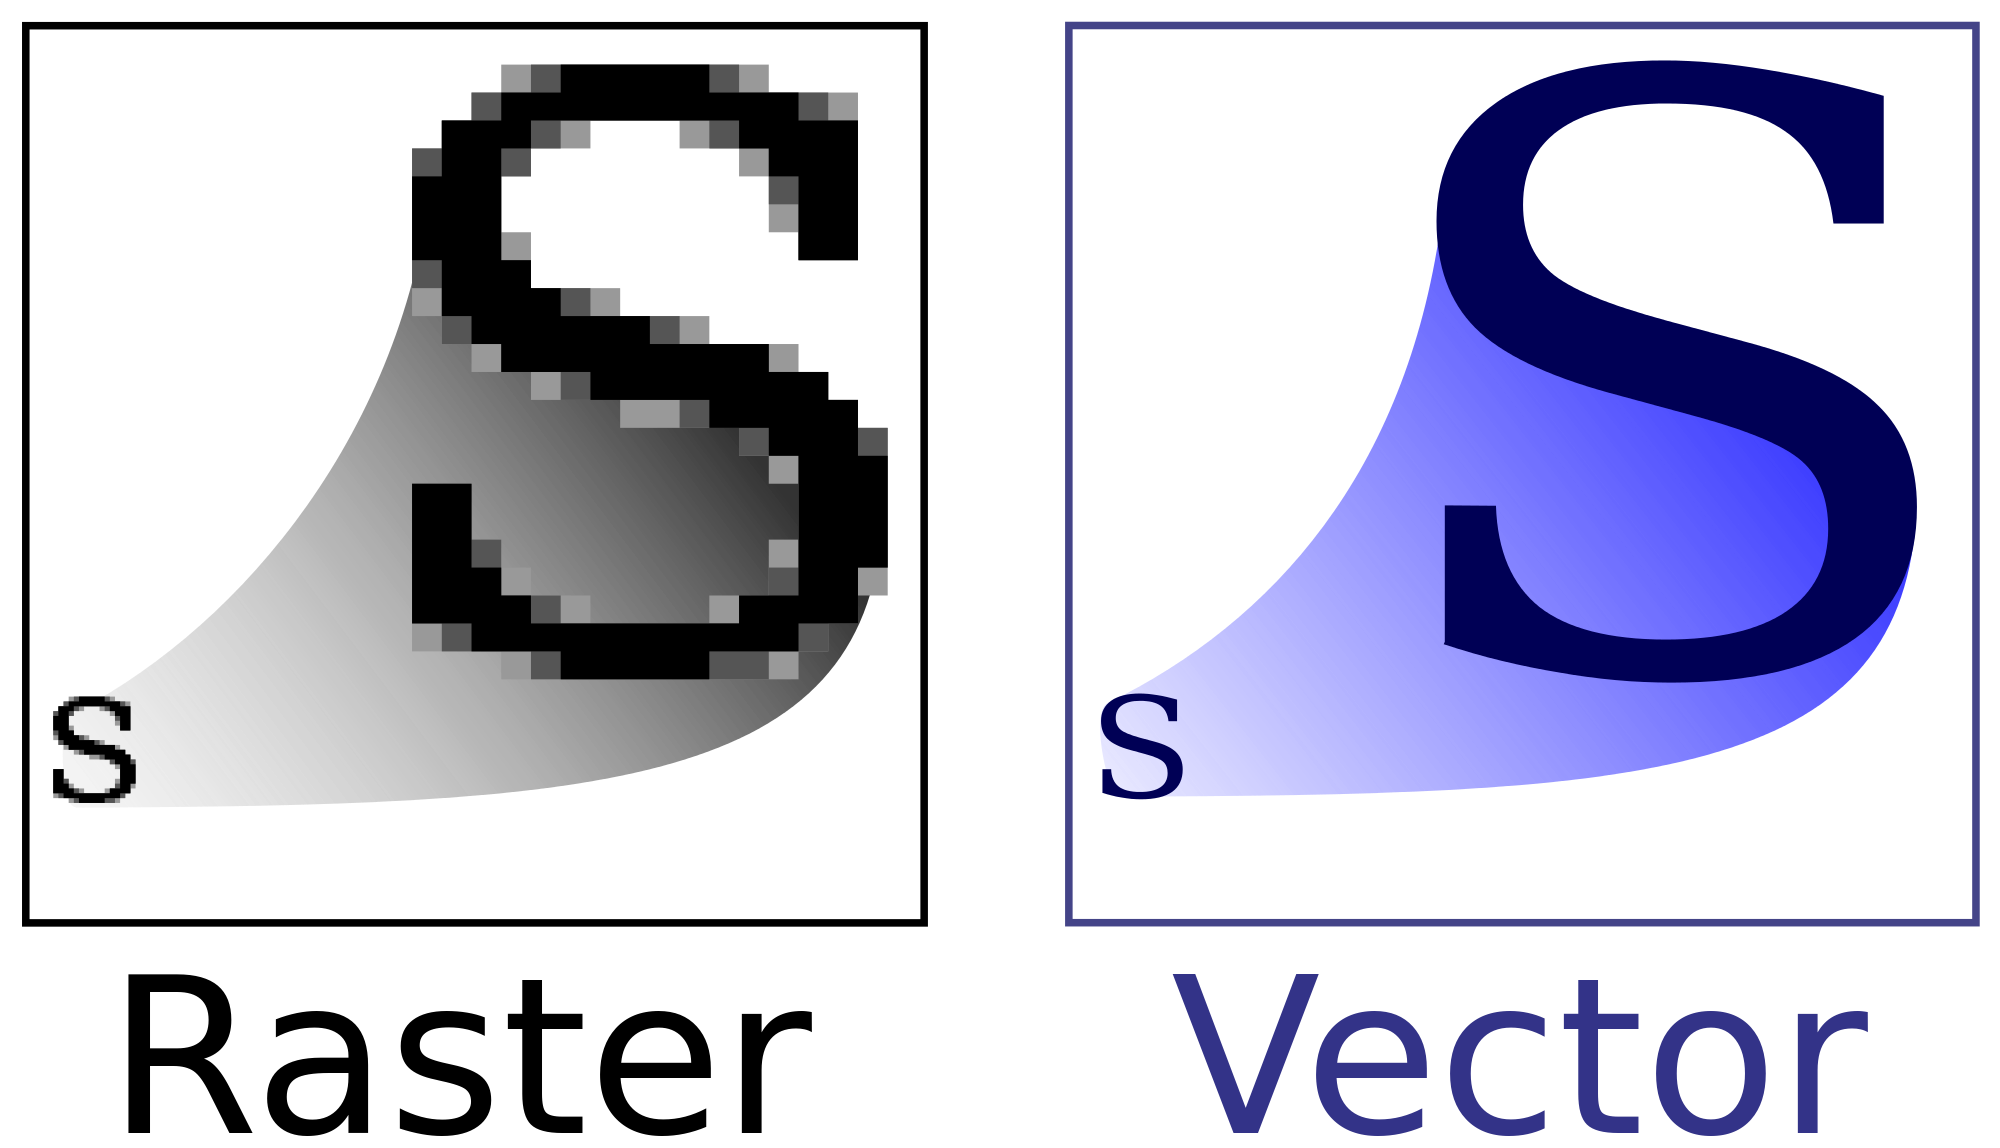
\includegraphics[width=0.5\linewidth]{images/bm_vs_svg.png}
\caption{Scaling comparison between raster graphics and vector graphics \cite{svg}.}
\label{fig:vectorscaling}
\end{figure}

Due to the geometrical nature of vectors, and the non-geometrical nature of the real world, it's not practical to use vector graphics to represent photographs.
Computer generated text, drawings or imagery, for use in graphical design, are the most common use case for vector graphics today, since the graphics can easily be scaled up or down by demand.
Most professional image processing and design software, e.g. Adobe Illustrator, support vector graphics.
At the time of writing, \texttt{svg} and \texttt{ai} are two examples of commonly used vector formats.

%In vector graphics an image is created by assembling a set of figures into a more complex image.
%These base figures are for example lines, circles, ellipses or curves. //TODO: Maybe reformat this

\subsubsection{Bézier curves}
\label{sec:bezier}
A popular type of curve in vector graphics is the Bézier curve.
Bézier curves can represent everything from a straight line to very complex paths with a lot of turns and changes in direction.
A Bézier curve is defined by a series of control points ranging from \(P_0\) to \(P_n\).
n is called the order of the curve and as such you end up with linear (n = 1), quadratic (n = 2), and cubic (n = 3) Bézier curves.
Formulas for Bézier curves with n=1,2,3 are shown in Equation \ref{equ:line} to \ref{equ:cube}.
B(t) is the point on the curve at t.
As t can be incremented as little or as much as wanted points on the curve can be calculated as granularly as desired.

\begin{cequation}[H]
	\begin{equation}
	    \label{equ:line}
		\mathbf{B}(t)=\mathbf{P}_0 + t(\mathbf{P}_1-\mathbf{P}_0)=(1-t)\mathbf{P}_0 + t\mathbf{P}_1 \mbox{ , } 0 \le t \le 1
	\end{equation}
	\caption{Linear Bézier curve}
\end{cequation}

\begin{cequation}[H]
	\begin{equation}
		\mathbf{B}(t) = (1 - t)^{2}\mathbf{P}_0 + 2(1 - t)t\mathbf{P}_1 + t^{2}\mathbf{P}_2 \mbox{ , } 0 \le t \le 1
	\end{equation}
	\caption{Quadratic Bézier curve}
\end{cequation}

\begin{cequation}[H]
	\begin{equation}
	    \label{equ:cube}
		\mathbf{B}(t)=(1-t)^3\mathbf{P}_0+3(1-t)^2t\mathbf{P}_1+3(1-t)t^2\mathbf{P}_2+t^3\mathbf{P}_3 \mbox{ , } 0 \le t \le 1
	\end{equation}
	\caption{Cubic Bézier curve}
\end{cequation}

\subsection{Vector Graphics in Modern Computing}

Vector graphics is not in frequent use today as a display technology, however it is widely used to represent data internally in a computer.
Two examples of vector technology in use today are the SVG format and text in TrueType \cite{truetype}.

Apple Inc. \cite{apple} uses vector graphics in their drawing engine that is available to all iOS and OS X application developers.
This drawing engine is called Quartz 2D \cite{quartz2d} and is widely used in order to make resolution independent user interfaces.

\subsection{3D Graphics}
//TODO: Is this section needed?
Vector graphics are predominantly used to describe 2D graphics, in order to distinguish them from 2D raster graphics. 
In 3D graphics, most implementations utilize points, lines and curves to define shapes, which makes them a lot like vector graphics. 
Voxel graphics is an implementation of 3D graphics that tries to define it's shapes by utilizing three dimensional pixels, so-called 'voxels', but is rarely used.

\section{Display Technology}
In the early days of computer display, vector displays were mainly used.
The use of frame buffers started when transistor-based \gls{ram} was introduced.
As a result, raster graphics and displays were created. \cite[sec. 1.1]{graphics-visualization-algorithms}.

Today, there exists a vast variety of display technologies - a few examples are \gls{crt}, \gls{lcd}, \gls{led} and \gls{oled}.
This section discusses vector displays and raster displays, and follows with a comparison between the two. It ends with an introduction to an oscilloscope, which was used in the project to output the vector graphics.

\subsection{Raster Display}
There exists a variety of raster display technologies, however they have a few common attributes.

Raster graphics uses a tecnique called frame buffer.
A frame buffer is used to hold the current image.
When the screen is ready to read a new image, this is done from the frame buffer.
After the image has arrived, the images scanned line by line.
The scan is done from top to bottom of the image.

\subsection{Vector Displays}
A vector display/monitor displays graphics by drawing from point to point. 
All vector displays utilize CRT (Cathode Ray Tube) technology, which contain one or more electron emitters that fire electron beams that are deflected onto a phosphorescent screen to display images.

The basic vector display is monochromatic. 
However, certain displays with color support exist. 
By using a shadow mask - that is a perforated plate that acts as a filter - between the electron guns and the screen, different colors can be displayed. This is achieved by having one electron gun for red, green and blue. Each gun shoots electron at different angles through the mask, and different intensities for each gun can create different colors.

Vector displays are pretty much obsolete today, because of raster screens' inexpensiveness and support for graphics with a higher level of detail. 
Also, vector graphics can - with modern algorithms - efficiently be translated to raster graphics, called rasterisation.
Translating raster graphics to vector graphics, however, is a complex process.

// TODO: Maybe a few references for these statements?
\subsection{Display Comparison}
The main difference between vector and raster displays, is that vector displays draws the image by scanning primitives, and a raster display draws the image by using scanlines. 

While a CRT raster display scans repeatedly in a fixed pattern, a vector display scans lines by gradually firing the electron beam to a point defined by two voltages: one defining the horizontal placement X and one defining the vertical Y. 
Once a line is drawn, the electron emitter stops firing and moves to the starting point of the next line, thus leaving out dark areas. 
This process is shown in figure \ref{fig:vectorscan}.

Since vector displays are able to draw directly from one point to another, they do not suffer from artifacts such as aliasing and pixelation, which are present in raster displays\cite{vector-monitor}.
However, graphic complexity on vector displays are very limited compared to raster screens.

\begin{figure}[h!]
\centering 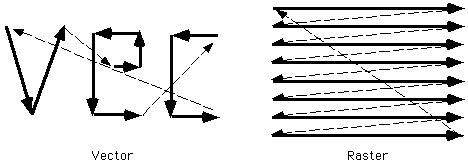
\includegraphics[width=0.8\linewidth]{images/scan.png}
\caption{Scan comparison between vector graphics (left) and raster graphics (right)\cite{vecvsras}.}
\label{fig:vectorscan}
\end{figure}

After an image has been drawn, both display types need to make the image stay put so that it can be perceived by humans. 
Some CRT displays use phosphor types that fade out very quickly and needs redrawing 30-40 times per second\cite{vector-monitor}.
However, special types of phosphor can last for several minutes.
//TODO: why is TFT introduced here? would LCD suffice? Modern Raster displays have the advantage that once an image has been 'configured' in the TFT display, it remains as long as the display is powered. 
Thus, no constant redrawing is necessary. //TODO: Unsure about this, fact check please!
Moving images are nothing more than successive images drawn to the display.

Screen flickering is an artifact caused by lower refresh rates than the human eye perceives as natural motion, and can occur in both display types. \cite{flicker}
On vector displays, the entire screen does not have to be scanned every time, only the areas that the electron beam has to light up.
However, the sometimes irregular electron beam motion is often slower than raster screens' predictable scanning.
Because of this, the refresh rate of a vector display is actually more limited, since it has no way of limiting the scene size. // Needs rewriting. Is 'limited' the right word?
When more primitives need to be drawn, the display will start to flicker more and more.
A raster display guarantees that all pixels will be updated within the required refresh rate, since the number of pixels always stays the same.

// TODO: Maybe a few references for these statements?

\subsection{Oscilloscope}
An oscilloscope is a popular lab tool used to output voltage as a function of time.
Modern oscilloscopes often use thin film transistor (TFT) displays and rasterize output. 
However, older models include a CRT vector display.

To draw on such an oscilloscope, the device must support at least two input channels, and the ability to draw in X-Y mode.
This means that two of the input channels (usually Ch1 and Ch2) governs the electron ray deflectors, which are controlled through electrostatics.
If the channels are provided with a constant voltage, a dot will be displayed on the screen - in contrast to normal mode, where a line would be drawn. // TODO: What is 'normal' mode? Varying voltage?

The voltage on channel one will normally decide the beam's horizontal X position, and channel two its vertical Y position.
To draw a line on the oscilloscope, frequent changes to the voltage of one or both channels is necessary to make the image remain on the screen. // For our osc this is true, but other types may be different
Changing the voltage on only one channel will produce a horizontal or vertical line.


\section{FPGA}
An \gls{fpga} was to be used to implement the processor.
The FPGA - an integrated circuit - is a powerful tool, in that it can be configured to support a wide array of use cases.
While a normal processor is application specific and configured during manufacturing, an \gls{fpga} includes programmable logic that can be configured almost any way you want it\cite{fpga}.
gls{hdl}s, e.g. VHDL and Verilog, are used to program the \gls{fpga}.
\gls{fpga}s provide both advantages and disadvantages compared to an \gls{asic}.
Most noteworthy is the simpler design cycles and a predictable project cycle, compared to the decreased customizability and higher unit costs for high volume productions \cite{fpgavsasic}.
